\section{Proportional-Integral-Derivative controllers}

PID controllers are commonly found in industrial control systems, where their
task is to correct the state of a process, based on its measured error against
a target state. The correction is calculated based on the proportional,
integral and derivative of the error function, thus giving it this name.

\begin{figure}[h]
	\centering
	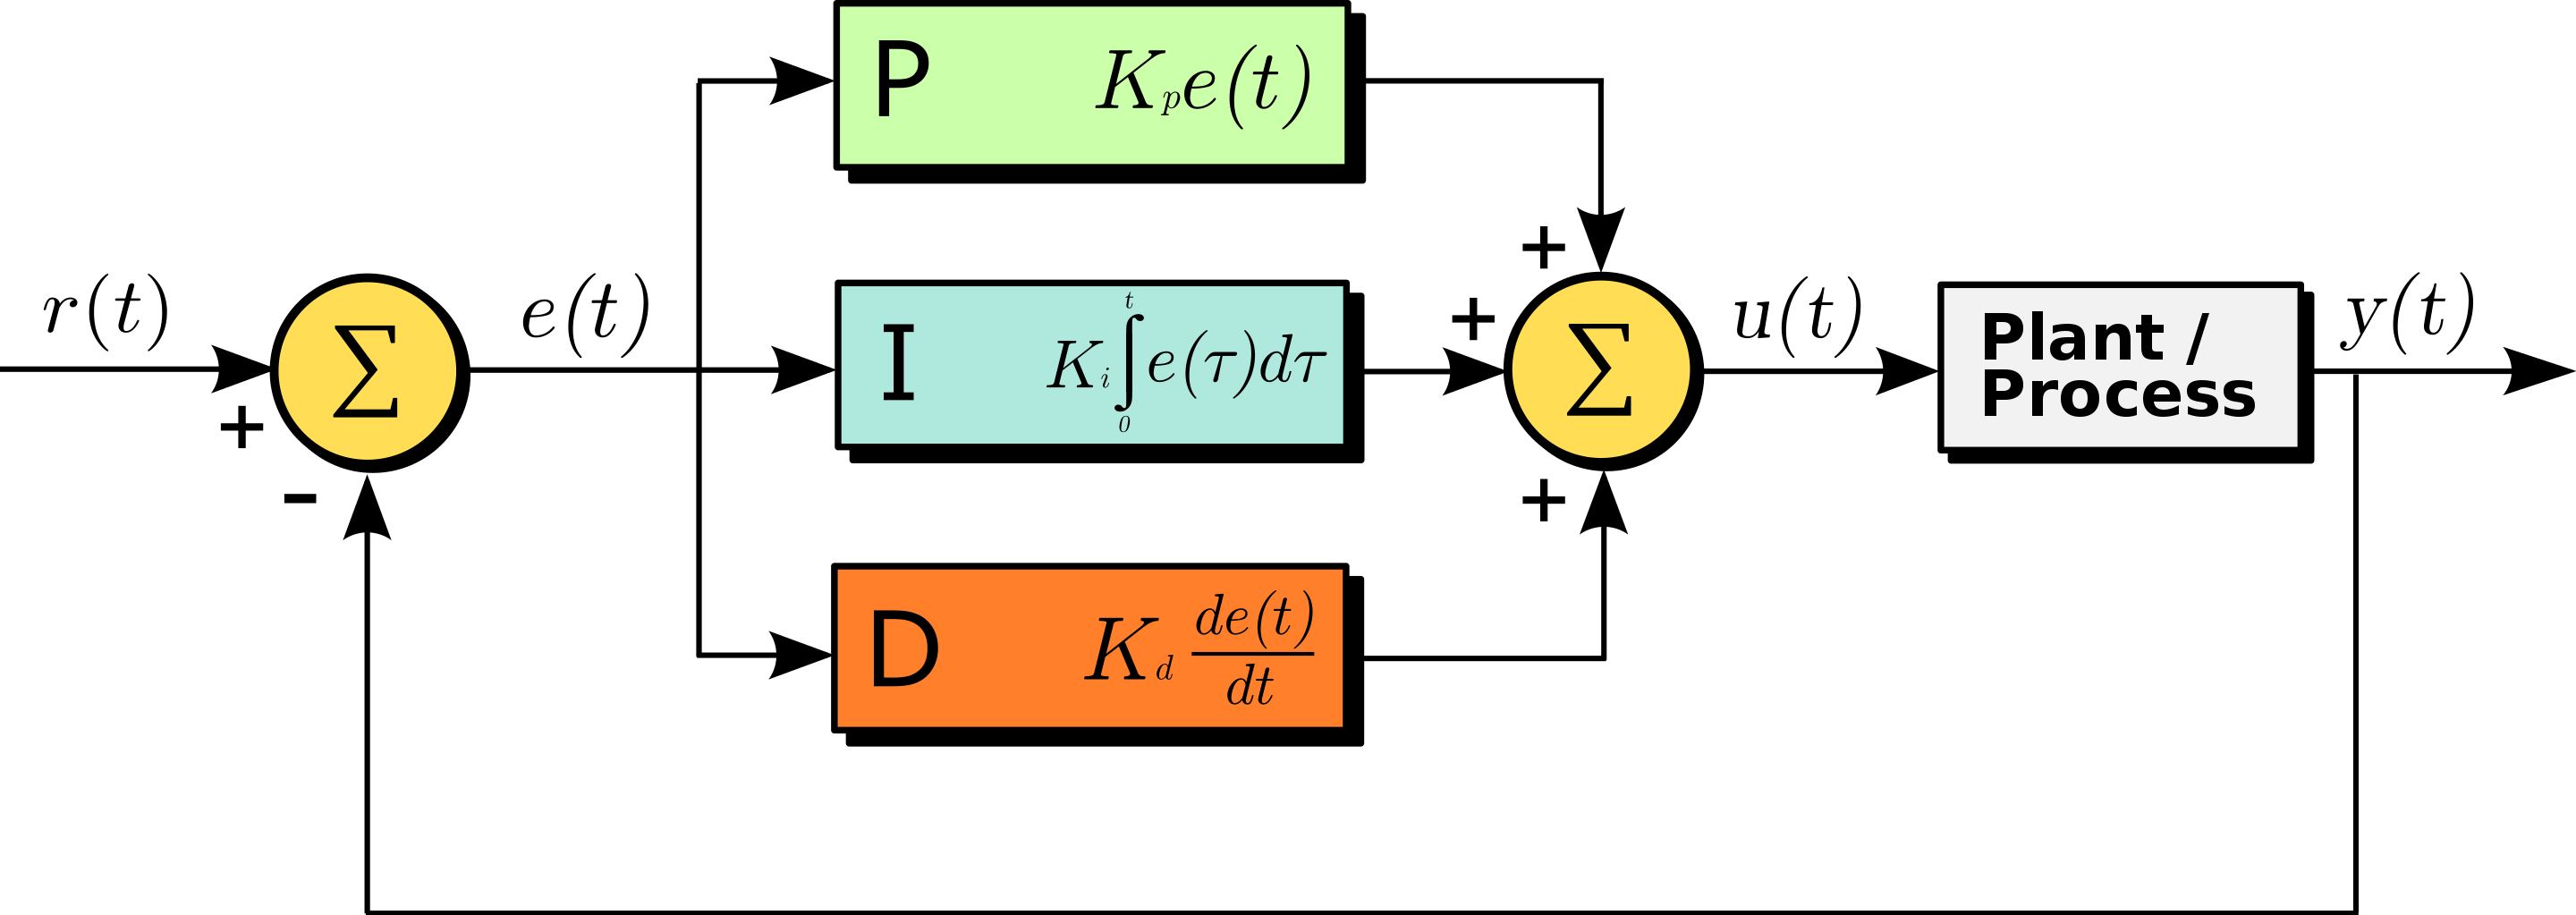
\includegraphics[width=0.9\textwidth]{figure/pid.png}
	\caption{The feedback loop of a PID controller.}
	\label{fig:pid-loop}
\end{figure}

The PID controller can be expressed mathematically as

\begin{equation}
	u(t) = k_p e(t) + k_i \int\limits_0^t e(t^{\prime}) dt^{\prime} + k_d \frac{de(t)}{dt}
\end{equation}

where $k_p$, $k_i$, and $k_d$ are the coefficients of the proportional,
integral and derivative terms, respectively, and $e(t)$ is the error at time
$t$.

The error function is typically the difference between the desired setpoint,
and the current setpoint. The three terms need to be properly weighted, through
fine-tuning of their respective gains, as to properly minimize the error
over time.

The first term, \emph{proportional}, is rather simple and intuitive: the
control command increases and decreases in proportion to the error. In essence,
a simple proportional control can be used by itself; the remaining terms help
compensate for cases where the controlled system cannot be modeled linearly
in one dimension.

As for the \emph{integral}, the output command varies in gain with respect to
the error over time. Effectively, the longer an error perdures, the larger its
integral grows, which results in an increase in this term for the controller.

Finally, the \emph{derivative} term, as its name indicates, only reacts to the
rate of change in the error and does not damper the error at all by itself.
If used properly, it has the effect of attenuating the amplitude of the signal
computed by the other terms with the aim of preventing overshooting. However,
as in every derivative-based optimization algorithm, it can also be the cause
of this phenomenon if its coefficient is set too high.\\

For this specific implementation, there are in fact two independent PID
controllers: one for the $Z$-axis in the body frame and responsible for
vertical alignment, and a second one for the yaw rotation of the UAV. The
function responsible for calculating the two velocity components is shown in
the following listing:

\begin{lstlisting} 
Velocity PID::Compute(Vector3d err, Velocity current_velocity)
{
	this->err_integral += err * (1./this->rate);
	Vector3d err_derivative = -current_velocity.linear;
	double z = this->gain_z.at("p") * err.y
		+ this->gain_z.at("i") * this->err_integral.y
		+ this->gain_z.at("d") * err_derivative.z;

	double yaw = this->gain_yaw.at("p") * err.x
		+ this->gain_yaw.at("i") * this->err_integral.x
		+ this->gain_yaw.at("d") * -current_velocity.yaw;

	Vector3d linVel(this->x_velocity, 0, z);
	Velocity vel;
	vel.linear = linVel;
	vel.yaw = yaw;

	return vel;
}
\end{lstlisting}
